\section{Results}

\subsection{Motor Friction Estimation}
The viscous damping coefficient \( b \) was found to be \( 0.001 \) Nm/rad/s for the hip motors (A20 etc) and \( 0.0001 \) Nm/rad/s for the knee motors (A14 etc). Figures \ref{fig:results:motor_friction_estimation:linear_regression_knee_motor} and \ref{fig:results:motor_friction_estimation:linear_regression_hip_motor} show the linear regression fit of the pendulum data used to estimate these coefficients for the knee and hip motors respectively.

\begin{figure}[h]
    \centering
    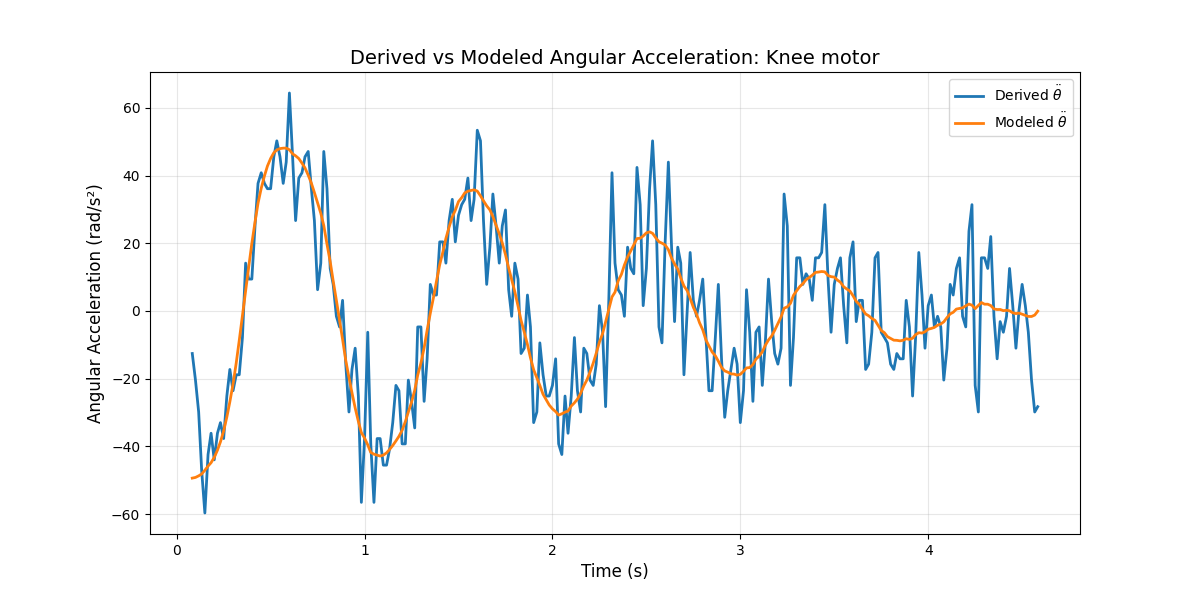
\includegraphics[width=0.8\textwidth]{Images/results/friction_est_knee_motor.png}
    \caption{Linear regression fit of the pendulum data. }
    \label{fig:results:motor_friction_estimation:linear_regression_knee_motor}
\end{figure}

\begin{figure}[h]
    \centering
    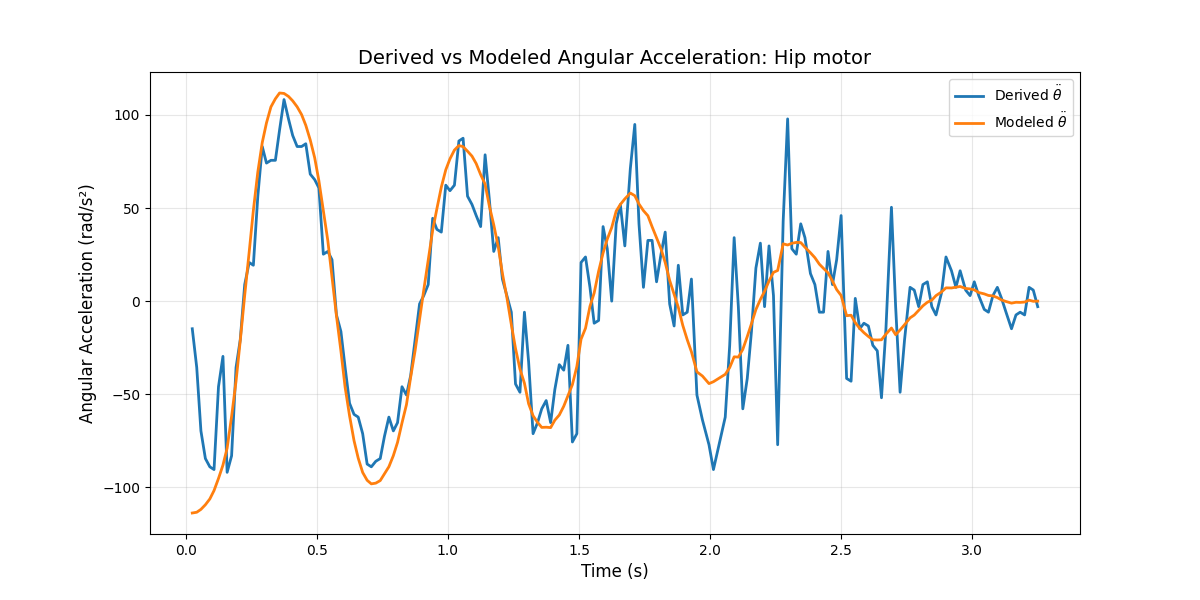
\includegraphics[width=0.8\textwidth]{Images/results/friction_est_hip_motor.png}
    \caption{Linear regression fit of the pendulum data. }
    \label{fig:results:motor_friction_estimation:linear_regression_hip_motor}
\end{figure}







\subsection{Link Length Optimization}
The grid search results for both Earth and Mars gravity are shown in figure \ref{fig:results:grid_search_results}. The search explored link length ratios from 0.5 to 2.0 and total lengths from 10cm to 40cm, in increments of 0.1 and 0.5cm respectively.
In the Earth gravity case, the highest jump height of 10.5cm was achieved with a link length ratio of 1.0 and a total length of 20cm, corresponding to L1=L2=10cm.  

\begin{figure}[h]
    \centering
    \includegraphics[width=0.8\textwidth]{Figures/results/grid_search_results_earth.png}
    \caption{Grid search results showing jump height performance across different link length configurations under Earth gravity.}
    \label{fig:results:grid_search_results}
\end{figure}

In the Mars gravity case, the highest jump height of 10.5cm was achieved with a link length ratio of 1.0 and a total length of 24cm, corresponding to L1=L2=12cm.
\begin{figure}[h]
    \centering
    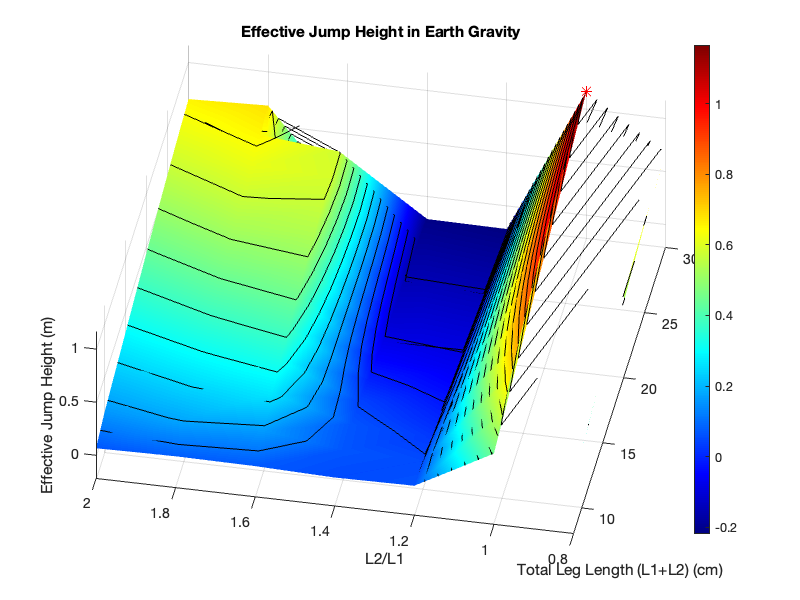
\includegraphics[width=0.8\textwidth]{Images/results/grid_search_results.png}
    \caption{Grid search results showing jump height performance across different link length configurations under Mars gravity.}
    \label{fig:results:grid_search_mars}
\end{figure}

In both Mars and Earth gravity, the optimal link length ratio is 1.0 across all total lengths, with steep drops in jump height for ratios under 1.0 and less steep drops for ratios over 1.0.

\subsection{Motor Only Jumping Performance}
Figure \ref{fig:results:grid_search_results} shows the grid search results for jumping performance without spring assistance, using only motor torque. The search used the same link length ratios and total lengths as the spring-assisted search.

\begin{figure}[h]
    \centering
    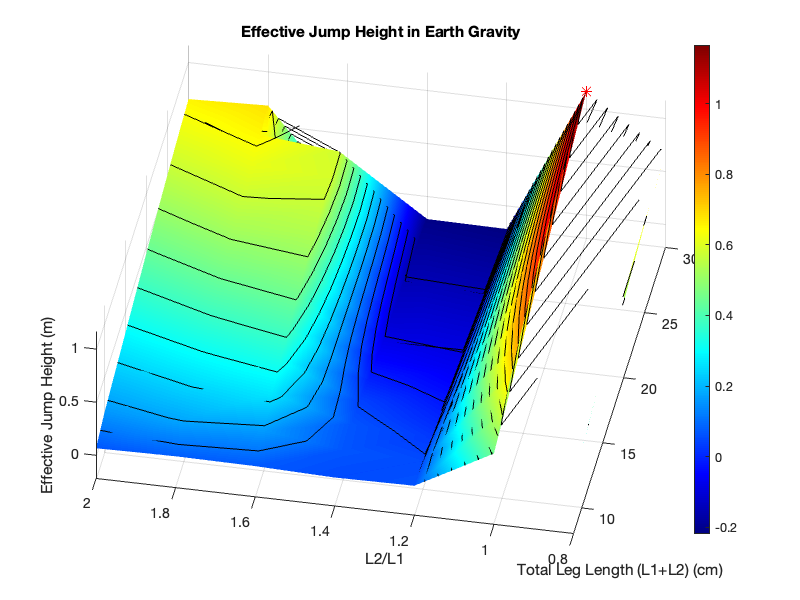
\includegraphics[width=0.8\textwidth]{Images/results/grid_search_results.png}
    \caption{Grid search results showing jump height performance using only motor torque, without spring assistance.}
    \label{fig:results:motor_only_grid_search}
\end{figure}
